\section{Corpus study}
\label{sec:corpusstudies}

\subsection{Preliminaries}

\subsubsection{Corpus choice}
\label{sec:gettingdata}

For the present study, I used the 21 billion token German \textit{Corpus from the Web} (COW) in its 2014 version DECOW14A (\citealp{SchaeferBildhauer2012full}, and \citealp{Schaefer2015b}, as well as \citealp{BiemannEa2013}, and \citealp{SchaeferBildhauer2013}, for overviews of web corpora in general and the methodology of their construction).%
\footnote{The COW corpora (Dutch, English, French, German, Spanish, Swedish) are made available for free at \url{https://www.webcorpora.org}.
At the time of this writing, a newer 2016 version DECOW16A has already been released.}
This corpus was chosen first because the external validity of any study is increased through a more heterogeneous sample \citep[30]{MaxwellDelaney2004}.
DECOW14A clearly has a much more heterogeneous composition compared with the only other very large corpus of German, the DeReKo of the Institute for the German Language \citep{KupietzEa2010}.
DeReKo contains almost exclusively newspaper texts.%
\footnote{It was shown in \cite{BildhauerSchaefer2016} that, for example, the range of topics is much smaller in DeReKo than in DECOW14A.}
The second reason for choosing this particular corpus is that normative grammars often adopt clear positions regarding the grammaticality of either the \NACa\ or the \PGCa.
Thus, newspaper text or any other texts which conform strongly to normative grammars may not represent the alternation phenomenon fully and without bias because authors and proofreaders who must adhere to normative guidelines might explicitly favour one alternative over another.
Web corpora, on the other hand, contain a significant amount of non-standard language from forums and similar sources.
For such reasons, COW corpora have been used in a number of peer-reviewed publications \citep{VanGoethemHiligsmann2014,VanGoethemHuening2015,MuellerS2014,Schaefer2016c,SchaeferSayatz2014,SchaeferSayatz2016,Zimmer2015}.


\subsubsection{Bootstrapping pairs of lemmas}
\label{sec:bootstrappinlemmapairs}

Among the factors potentially influencing the alternation (see Section~\ref{sec:germanmeasurenps}) are lemma-specific effects.
Therefore, it was necessary to obtain a sample in which most of the highly frequent actually-occurring combinations of kind nouns and measure nouns were represented.
Hence, I applied a two-stage process in order to obtain a list of co-occurring measure nouns and kind nouns.

In the first step, I exported a list of all nouns from the DECOW14A01 sub-corpus (one billion tokens large).
Then, the one hundred most frequent mass nouns were extracted manually from this list.
Mass nouns were defined as concrete nouns which genuinely denote a substance, combine with uninflected mass quantifiers such as \textit{viel} `much' and \textit{wenig} `little' (\textit{viel Bier} `much beer'), and form only sortal and unit plurals (such as the plural \textit{Biere} `types of beer' or `glasses of beer').
Abstract nouns which partially behave as mass nouns (for example, \textit{Spaß} `fun’ or \textit{Gefahr} `danger’) were excluded because they are not measured in the same way as concrete mass nouns.

This list of mass nouns was used in the second step to derive a list of measure nouns co-occurring with the mass nouns. 
In order to generate this list, I utilised the fact that a direct sequence of two nouns almost always instantiates the \NACb\ if the second noun is a mass noun.
I searched for all sequences N\Sub{1}N\Sub{2} where N\Sub{2} was one of the mass noun lemmas extracted in the first step.
Then, the resulting 100 lists of noun-noun combinations were each sorted by frequency in descending order and sieved manually to remove erroneous hits.
From each of the 100 lists, I also removed noun-noun combinations that had a frequency below 2, except if the individual list would have otherwise been shorter than 20 noun-noun combinations.
The result was a list of the most frequent 2,365 individual combinations of measure and mass nouns.

\subsubsection{Variables and annotation}
\label{sec:variablesandannotation}

The full set of manually annotated variables for the main study is given in Table~\ref{tab:variables}.%
\footnote{All numeric variables were z-transformed to facilitate their interpretation in the regression models.}
Notice first that \textit{Construction} is the response variable with the values \textit{PGCadj} and \textit{NACadj}.

\begin{table}
  \centering
  \begin{tabular}{llll}
    Unit of reference & Variable                      & Type    & Levels (for factors only) \\
    \midrule
    Document       & Badness                          & numeric &                           \\
                   & Genitives                        & numeric &                           \\
    Sentence       & Cardinal                         & factor  & Yes, No                   \\
                   & \textbf{Construction (response)} & factor  & NACadj, PGCadj            \\
                   & Measurecase                      & factor  & Nom, Acc, Dat             \\
    Kind lemma     & Kindattraction                   & numeric &                           \\
                   & (Kindcollo)                      & numeric &                           \\
                   & Kindfreq                         & numeric &                           \\
		   & Kindgender                       & factor  & Masc, Neut, Fem             \\
    Measure lemma  & Measureattraction                & numeric &                           \\
                   & (Measurecollo)                   & numeric &                           \\
                   & Measureclass                     & factor  & Physical, Container,      \\
                   &                                  &         & Amount, Portion, Rest     \\
                   & Measurefreq                      & numeric &                           \\
  \end{tabular}
  \caption{Annotated variables for the corpus studies}
  \label{tab:variables}
\end{table}

The variables \textit{Kindattraction} and \textit{Measureattraction} encode the ratio with which a given kind noun lemma or measure noun lemma occurs in the \PGCd\ and the \NACb.
They were calculated from auxiliary samples to be described in Section~\ref{sec:mainstudysampling} as a log-transformed quotient.
The higher the value for some noun, the (relatively) more often this noun occurs in the \PGCd.
It could be argued that other measures of attraction strength should be used, for example those popularised in collostructional analysis (CA; \citealp{StefanowitschGries2003,GriesStefanowitsch2004}; see also \citealp{Gries2015a}).
However, the goal here is to quantify how often lemmas occur in the \PGCd\ and the \NACb, and these constructions do not compete at all but are rather mutually exclusive.
While this does not preclude the use of CA, it is an open question whether the marginals are cognitively relevant in this case.
After all, the main difference between the quotient used here and measures used in CA (originally signed logarithmised p-values from a Fisher test) is that they take the marginals into account. 
However, using Fisher-p-based collexeme strength instead of the raw frequency quotient was tried as an alternative (variables \textit{Kindcollo} and \textit{Measurecollo}).
See Section~\ref{sec:mainstudystatisticalmodel} for a discussion of the negative results.

In Section~\ref{sec:analyses}, it was hypothesised that classes of measure lemmas might have different preferences for the two alternants.
To capture this, class information was annotated for measure lemmas as \textit{Measureclass}.
The variable \textit{Cardinal} encodes whether the MNP is modified by a cardinal.

To capture the influence of style mentioned in Section~\ref{sec:analyses}, two proxy variables were used.
At the document level, the DECOW14A corpus has an annotation for \textit{Badness}.
As described in \cite{SchaeferEa2013}, \textit{Badness} measures how well the distribution of highly frequent short words in the document matches a language model of standard German.
The paper also shows that the Badness score corresponds robustly with human raters' intuitions about text coherence and text quality.
Documents with higher Badness usually contain more incoherent language and shorter sentences.
If the \PGCa\ actually favours more elaborate stylistic levels, a high \textit{Badness} should be correlated with fewer occurrences.
Documents in DECOW14 have also been annotated with a variable called \textit{Genitives}.
For each document it is the case that the higher the values of this variable, the lower the proportion of genitives among all case-bearing forms.
A high number of genitives is also indicative of a more formal, elaborate style close to the written standard.
However, since the \PGCa\ contains a genitive itself, the regressor variable \textit{Genitive} and the document-level variable \textit{Genitives} are not fully independent.
Since instances of the \PGCa\ make up for only a minute fraction of all genitives, I still use \textit{Genitives} as a regressor with the appropriate caveats.

Furthermore, to control for simple frequency effects, \textit{Kindfreq} and \textit{Measurefreq} are included as the logarithm-transformed frequencies per 1,000,000 words of each lemma, extracted from the frequency lists distributed by the DECOW14A corpus creators on their web page.

Finally, two variables have been added as nuisance variables in the context of the present study.
First, the case of the measure noun was manually annotated (variable \textit{Measurecase}).
This was carried out because it was reported in the literature that MNPs in the dative containing a masculine or neuter kind noun favour the \PGCa\ more than the corresponding nominative and accusative MNPs \citep{Hentschel1993,Zimmer2015}.
As an example, \textit{mit einem Stück frischen Brots} `with a piece of fresh bread' (\PGCa) would be preferred more strongly against \textit{mit einem Stück frischem Brot} (\NACa).
As with all the examples, native speakers of German will most likely notice that differences are subtle.
Second, due to differences in case syncretisms, it is likely that feminine kind nouns have slightly different preferences than masculine and neuter ones, and hence the appropriate variable \textit{Kindgender} was annotated.

\subsection{Pre-study: main prototype effects in the non-alternating constructions}
\label{sec:prestudy}

The main study to be reported below deals exclusively with the alternating constructions, as is customary in alternation modelling.
However, the prototypical features described in Section~\ref{sec:prototypeeffects} should be observable in the non-alternating cases as well.
Therefore, in this section I examine the distribution of the prototypical features in the non-alternating cases to see whether they are in accord with the theoretical predictions.

\subsubsection{Sampling and annotation}

For this pre-study, each of the 2,365 combinations of measure noun lemma and kind noun lemma were queried in the \NACb\ and the \PGCd\ with a limit of 100 randomly chosen results for each single query.%
\footnote{The data package for this paper (including all concordances and R scripts) is made available under the following DOI\slash URL: \url{https://dx.doi.org/10.5281/zenodo.1254871}.}
From the resulting 35,766 sentences, 5,000 were randomly sampled for the statistical analysis.
All features described in Section~\ref{sec:variablesandannotation} were annotated except for the ones which do not apply in the non-alternating case (\textit{Kindattraction}, \textit{Measureattraction}, and \textit{Measurecase}).

\subsubsection{Statistical model}

The annotated concordance was analysed in the form of a multilevel logistic regression model using R \citep{R} and the \textit{lme4} package \citep{Bates2010,BatesEa2015}.
An alternative \textit{BOBYQA} optimiser from the \textit{nloptr} package \citep{Johnson2017} was used for all fits with \textit{lme4} reported in this paper.

\begin{table}
  \centering
  \resizebox{\textwidth}{!}{
    \begin{tabular}{llrlrrrc}
    Model level  & Regressor         & $\text{p}_{\text{PB}}$ & Factor level & Coefficient & CI low & CI high & CI excludes 0 \\
    \midrule
    1                & Badness           & 0.042                  &              &  0.120      & -0.002 &  0.228  &              \\
                     & Cardinal          & 0.001                  & No           &  1.419      &  0.869 &  1.993  &  *           \\
                     & Genitives         & 0.001                  &              & -0.710      & -0.815 & -0.556  &  *           \\[0.5\baselineskip]

    
    2 (Kindlemma)    & (Kindfreq)        & (0.781)                &              &             &        &         &              \\
                     & (Kindgender)      & (0.199)                &              &             &        &         &              \\[0.5\baselineskip]
    
    2 (Measurelemma) & Measureclass      & 0.005                  & Container    & 0.445       & -0.579 &  1.532  &              \\
                     &                   &                        & Rest         & 1.745       &  0.649 &  2.831  &  *           \\
                     &                   &                        & Amount       & 1.597       &  0.125 &  2.751  &  *           \\
                     &                   &                        & Portion      & 1.782       &  0.771 &  2.690  &  *           \\
                     & (Measurefreq)     & (0.265)                &              &             &        &         &              \\

  \end{tabular}
  }
  \caption{Coefficient table with 95\% bootstrap confidence intervals for the pre-study; the intercept is -5.370}
  \label{tab:smalltable}
\end{table}

The coefficient estimates are specified in Table~\ref{tab:smalltable} for each regressor (column \textit{Coefficient}).
Given the coding of the response variable, coefficients leaning to the positive side can be interpreted as characterising a configuration typical of the \PGCd.
For a robust quantification of the precision of the estimation, I ran a parametric bootstrap (using the \mbox{\textit{confint.merMod}} function from \textit{lme4}) with 1,000 replications and using the percentile method.
The resulting 95\% bootstrap confidence intervals are reported in Table~\ref{tab:smalltable} (columns \textit{CI low} and \textit{CI high}).
The column \textit{CI excludes 0} shows an asterisk for those intervals that do not include 0.
Furthermore, for each regressor, a p-value was obtained by dropping the regressor from the full model, re-estimating the nested model, and comparing it to the full model.
Instead of inexact Wald approximations and Likelihood Ratio Tests, I used a drop-in bootstrap replacement for the Likelihood Ratio Test in the form of the function \textit{PBmodcomp} from the \textit{pbkrtest} package \citep{HalekohHojsgaard2014}.
I call the corresponding value $p_{\text{PB}}$ (column $p_{\text{PB}}$).
Regressors which did not reach sig=0.05 in in the PBmodcomp test (\textit{Kindfreq}, \textit{Kindgender}, and \textit{Measurefreq}) were removed from the model, appear in brackets in Table~\ref{tab:smalltable}, and have no coefficient estimates.

The overall intercept is -5.370, and it represents \textit{Cardinal=Yes}, \textit{Measureclass=Physical} and 0 for all (z-transformed) numeric regressors.
The standard deviation of the random intercepts is 1.157 for \textit{Measurelemma} ($p_{\text{PB}}=0.001$) and 0.923 for \textit{Kindlemma} ($p_{\text{PB}}=0.002$).
Nakagawa \& Schielzeth's pseudo-coefficients of determination are $R_m^2=0.278$ and $R^2_c=0.566$ (\citealp{Gries2015}; \citealp{NakagawaSchielzeth2013}).

\subsubsection{Interpretation}

The coefficients of determination indicate that the influence of the fixed effects (marginal $R^2$) is adequately strong, and that lemma-specific effects are equally strong with a difference between the two coefficients of 0.289.

The main prototypical factors \textit{Cardinal} and \textit{Measureclass} both pass the PBmodcomp test at sig=0.05 and play the expected role.
Non-referential physical measure nouns (such as \textit{Gramm} `gram' or \textit{Liter} `litre') with a high degree of grammaticalisation favour the \NACb.
At the other end of the scale, nouns denoting natural portions like \textit{Haufen} `heap', \textit{Bündel} `bundle', \textit{Schluck} `gulp' favour the \PGCd.
Also, The presence of a cardinal modifier clearly favours the \NACb.
The stylistic factor \textit{Genitives} shows the predicted influence inasmuch as a general lack of genitives (which is encoded as a \textit{higher} value of the variable) favours the \NACb.
\textit{Badness} points into the wrong direction, but it barely reaches sig=0.05, and its confidence interval includes 0.
The lemma frequency regressors both clearly fail the PBmodcomp test.
I will return to these results in Section~\ref{sec:mainstudyinterpretation}.

\subsection{Main study: the alternation}
\label{sec:annotation}
\label{sec:corpushierarchicalmodel}

\subsubsection{Sampling and annotation}
\label{sec:mainstudysampling}

For the main study, each of the 2,365 noun–noun combinations was queried in the alternating constructions \PGCa\ and \NACa\ using a sub-corpus of DECOW14A (slices DECOW14A01 to DECOW14A10 with a total size of 10 billion tokens).
For further manual annotation, a random sub-sample was generated.
For each mass noun, the concordance was downsampled randomly to maximally 100 sentences, which resulted in 6,843 sentences.
In the manual annotation, the sample was further reduced to 5,063 sentences due to removal of noisy material, erroneous hits, and uninformative cases where the measure noun was in the genitive, in which case the \NACa\ cannot be distinguished from the \PGCa.%
\footnote{In a similar fashion, the 100 most frequent measure nouns occurring with plural kind nouns were listed and queried, resulting in a sample of 871 sentences.
As stated in Section~\ref{sec:themeasurenounphrasealternation}, the \NACa\ is virtually never used with plural kind nouns, and this sample was not used except for quantifying the frequency of occurrence of the constructions (67 times \NACa\ and 794 times \PGCa).
The sample is distributed with the data package accompanying this paper.}

Finally, two auxiliary samples were also drawn.
As mentioned in Section~\ref{sec:analyses}, the distribution of the measure and kind noun lemmas in the \NACb\ and the \PGCd\ with a determiner will be modelled as factors influencing the alternation.
Therefore, all noun-noun pairs from the process described above were also queried in the two non-alternating constructions, resulting in 17,252 hits for the \PGCd\ and 315,635 hits for the \NACb.

\subsubsection{Statistical model}
\label{sec:mainstudystatisticalmodel}

\begin{figure}[hb!]
  \centering
  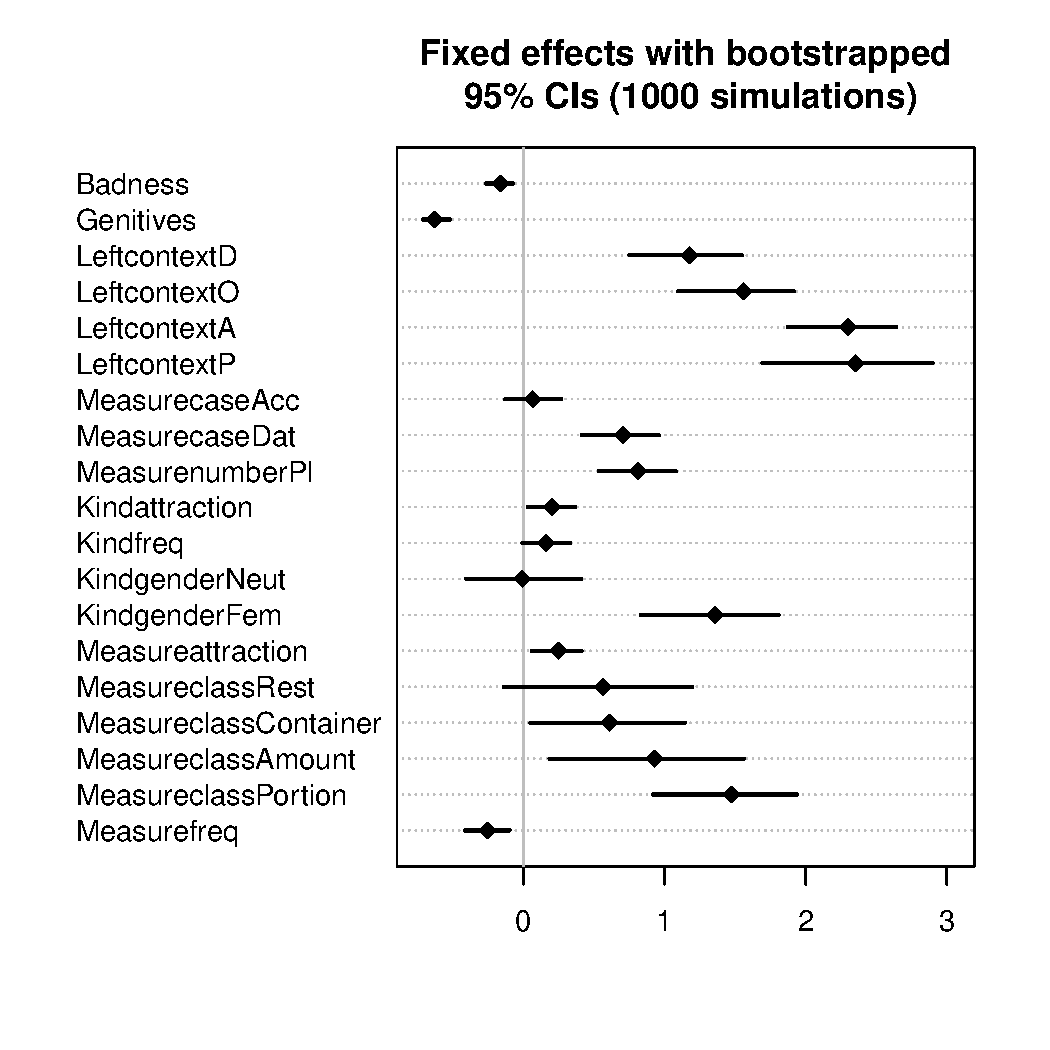
\includegraphics[width=0.85\textwidth]{../R/output/corpus_fixeffs}
  \caption{Coefficients with 95\% confidence intervals (for details see text); the intercept is -3.548}
  \label{fig:fixeffs}
\end{figure}

A multilevel logistic regression model was fit which models the influence of the regressors specified in Table~\ref{tab:variables} on the probability that the \PGCa\ is chosen over the \NACa.
All regressors from Table~\ref{tab:variables} were included, and the measure lemma and the kind noun lemma were specified as varying-intercept random effects.
The sample size was \textit{n=}5,063 with 1,134 cases of \PGCa\ and 3,929 cases of \NACa.
The results of the estimation are shown in Figure~\ref{fig:fixeffs} and in Table~\ref{tab:bigtable}.
The intercept estimated at -3.548 comprises \textit{Cardinal=Yes}, \textit{Measurecase=Nom}, \textit{Kindgender=Masc}, \textit{Measureclass=Physical}, and 0 for all numeric z-transformed regressors.

The regressors with the measure lemma as their unit of reference have no within-measure lemma variance, and the \textit{glmer} function automatically estimates them as group-level predictors (second-level effects), cf.\ \citet[265--269,302--304]{GelmanHill2006}.
The same goes for those listed with the kind lemma as their unit of reference.
Given the coding of the response variable, coefficients leaning to the positive side can be interpreted as favouring the \PGCa.

\begin{table}
  \centering
  \resizebox{\textwidth}{!}{
    \begin{tabular}{llrlrrrc}
    Model level  & Regressor         & $\text{p}_{\text{PB}}$ & Factor level & Coefficient & CI low & CI high & CI excludes 0 \\
    \midrule
    1               & Badness           &  0.002                 &              & -0.152      & -0.247 & -0.061  & *             \\
                    & Cardinal          &  0.001                 & No           &  1.189      &  0.862 &  1.466  & *             \\
                    & Genitives         &  0.001                 &              & -0.693      & -0.768 & -0.592  & *             \\
                    & Measurecase       &  0.001                 & Acc          &  0.030      & -0.150 &  0.212  &               \\
                    &                   &                        & Dat          &  0.705      &  0.455 &  0.944  & *             \\[0.5\baselineskip]
    
    2 (Kindlemma)   & Kindattraction    &  0.020                 &              &  0.225      &  0.049 &  0.393  & *             \\
                    & Kindfreq          &  0.095                 &              &  0.146      & -0.023 &  0.301  &               \\
                    & Kindgender        &  0.001                 & Neut         &  0.021      & -0.367 &  0.392  &               \\
                    &                   &                        & Fem          &  1.269      &  0.800 &  1.709  & *             \\[0.5\baselineskip]
    
    2 (Measurelemma) & Measureattraction &  0.001                 &              &  0.282      &  0.106 &  0.447  & *             \\
                    & Measureclass      &  0.001                 & Container    &  0.252      & -0.265 &  0.788  &               \\
                    &                   &                        & Rest         &  0.421      & -0.209 &  1.063  &               \\
                    &                   &                        & Amount       &  0.831      &  0.215 &  1.432  & *             \\
                    &                   &                        & Portion      &  1.217      &  0.675 &  1.684  & *             \\
                    & Measurefreq       &  0.005                 &              & -0.231      & -0.363 & -0.079  & *             \\

  \end{tabular}
  }
  \caption{Coefficient table with 95\% bootstrap confidence intervals for the main study; the intercept is -3.548}
  \label{tab:bigtable}
\end{table}

Standard diagnostics show that the model quality is quite good.
Nakagawa \& Schielzeth's pseudo-coefficients of determination are $R_m^2=0.409$ and $R^2_c=0.495$.
The rate of correct predictions is 0.843, which means a proportional reduction of error of $\lambda=0.297$.
Generalised variance inflation factors for the regressors were calculated to check for multicollinearity \citep{FoxMonette1992,ZuurEa2010}, and the highest corrected $\text{GVIF}^{1/2\text{df}}$ was 1.520 for \textit{Cardinal}.
The lemma intercepts have standard deviations of $\sigma_{\text{Measurelemma}}=0.448$ and $\sigma_{\text{Kindlemma}}=0.604$.
Only \textit{Kindfreq} ($\mpPB=0.095$) could be seen as slightly too high to be convincing, failing at sig=0.05.

The use of signed logarithmised Fisher p-values as a measure of collexeme strength (\textit{Measurecollo} and \textit{Kindcollo}) instead of the quotient for the attraction strength (\textit{Measureattraction} and \textit{Kindattraction}) (see Section~\ref{sec:variablesandannotation}) was not successful.
The $p_{\text{PB}}$ value for \textit{Kindcollo} was 0.191 and the one for \textit{Measurecollo} was 0.443.
The coefficients of determination dropped to $R_m^2=0.376$ and $R^2_c=0.480$.

\subsubsection{Interpretation}
\label{sec:mainstudyinterpretation}

\begin{figure}[h!]
  \centering
  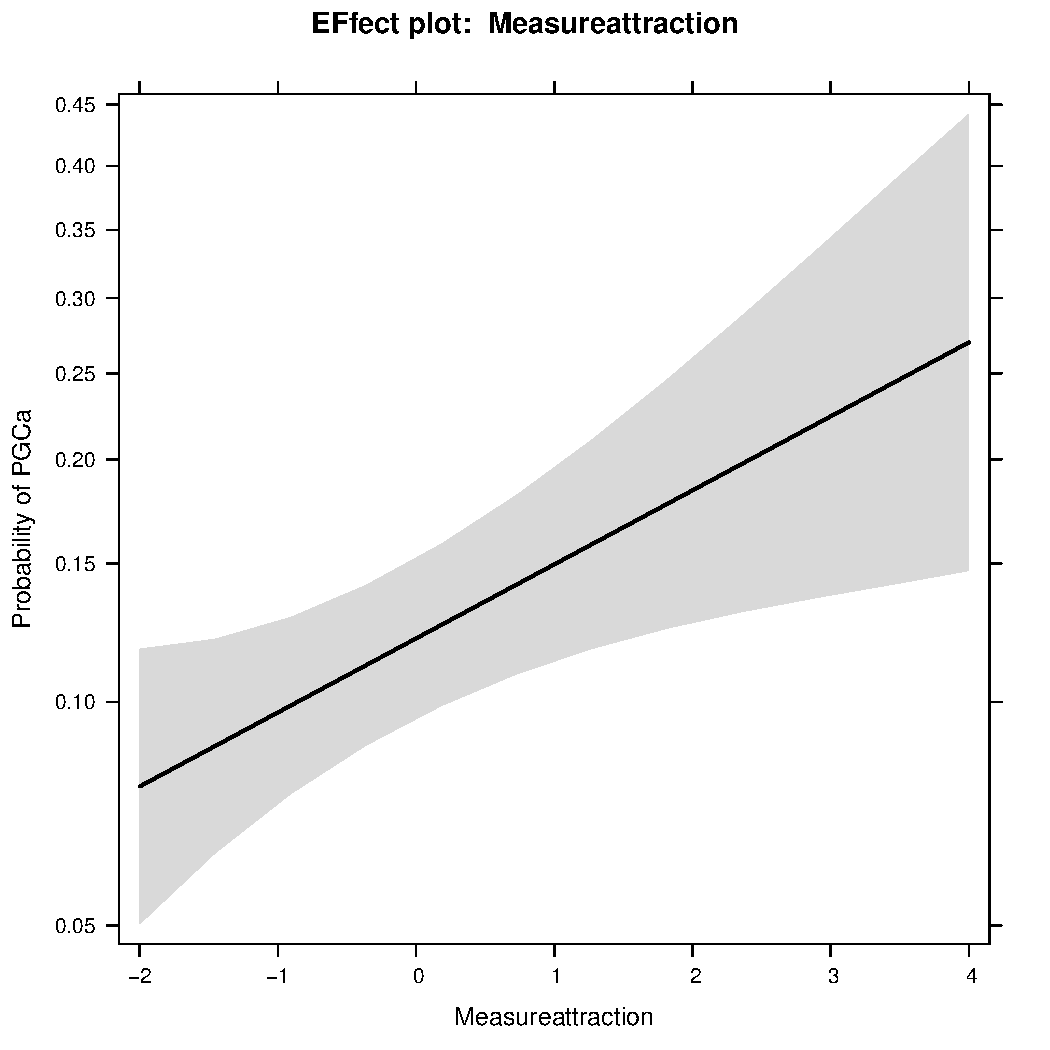
\includegraphics[width=0.5\textwidth]{../R/output/corpus_Measureattraction}~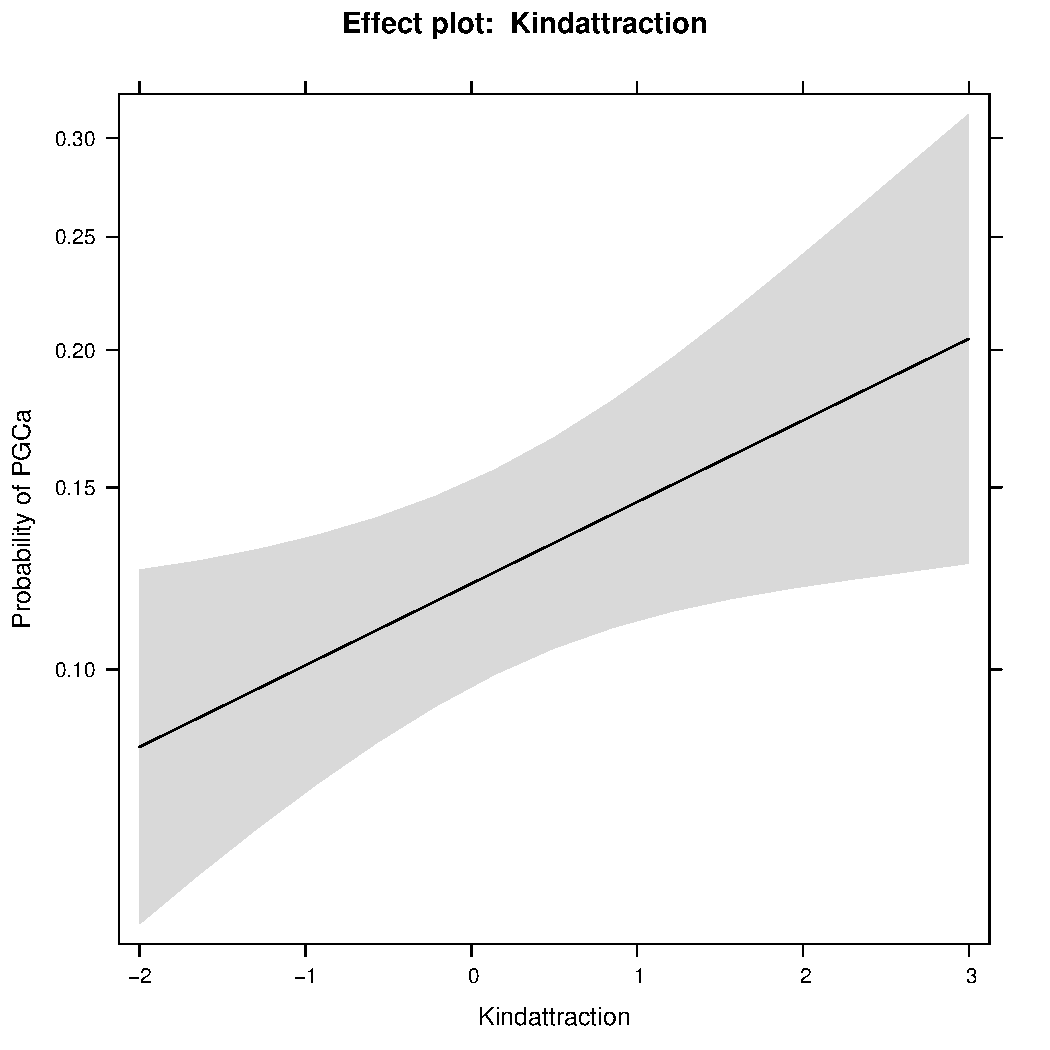
\includegraphics[width=0.5\textwidth]{../R/output/corpus_Kindattraction}
  \caption{Effect plots for the regressors \textit{Measureattraction} and \textit{Kindattraction}; y-axes are not aligned}
  \label{fig:eff:attraction}
\end{figure}

The results generally confirm the hypotheses from Section~\ref{sec:analyses}.
First, the exemplar effect (the influence of the non-alternating \PGCd\ and \NACb) was validated (see the effect plots in Figure~\ref{fig:eff:attraction}).%
\footnote{Effect plots were created using the \textit{effects} package \citep{Fox2003}.}
The effect is as expected:
if a lemma appears relatively more often in the \PGCd\ (compared to its frequency in the \NACb), the \PGCa\ tends to be chosen over the \NACa\ with this specific lemma.
The effect for measure nouns is even stronger and could be estimated with higher precision.

An interesting picture emerges for the lemma frequencies.
A higher-than-average lemma frequency of measure nouns favours the \NACa, which is as expected if we assume at least a tendency for highly grammaticalised words to be more frequent.
With kind nouns, higher frequency seems to favour the \PGCa.
However, this effect has no clear theoretical interpretation, and its coefficient estimate is imprecise (not reaching sig=0.05).
The effect can therefore be dismissed or treated as a nuisance variable.


\begin{figure}[h!]
  \centering
  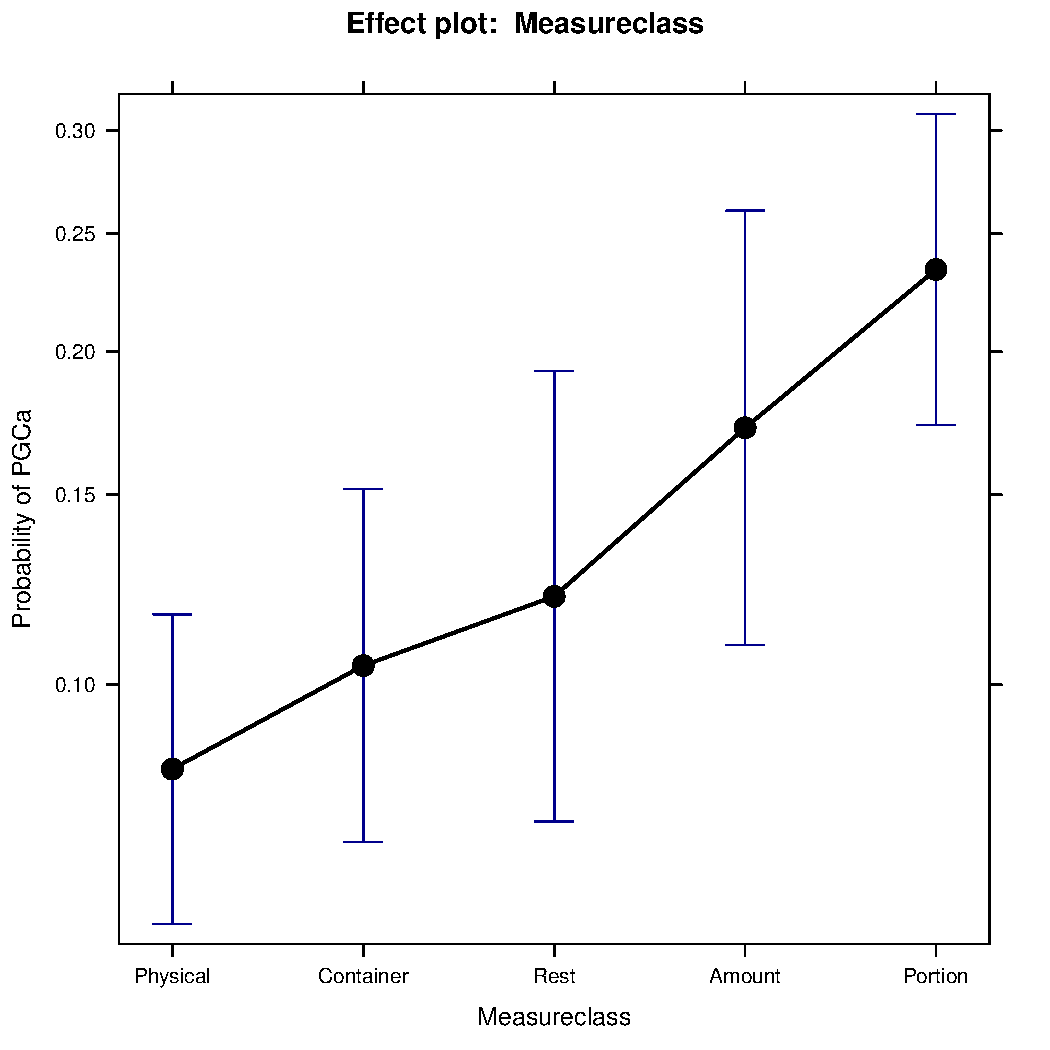
\includegraphics[width=0.5\textwidth]{../R/output/corpus_Measureclass}
  \caption{Effect plot for the regressor \textit{Measureclass}}
  \label{fig:eff:measureattraction}
\end{figure}

In Section~\ref{sec:analyses}, it was also hypothesised that classes of measure nouns with a higher degree of grammaticalisation should favour the \NACa.
The \textit{Measureclass} second-level predictor reaches sig=0.05 in the PBmodcomp test.
Looking at the effect plot in Figure~\ref{fig:eff:measureattraction}, it is evident that abstract non-referential physical measure nouns (such as \textit{Gramm} `gram' or \textit{Liter} `litre') with a high degree of grammaticalisation favour the \NACa.
At the other end of the scale, nouns denoting natural portions like \textit{Haufen} `heap', \textit{Bündel} `bundle', \textit{Schluck} `gulp' favour the \PGCa.
These are referential nouns, confirming the hypothesis that it is prototypical of the PGC to contain two referential nouns, while the NAC prototypically only contains one (the kind noun).

\begin{figure}[h!]
  \centering
  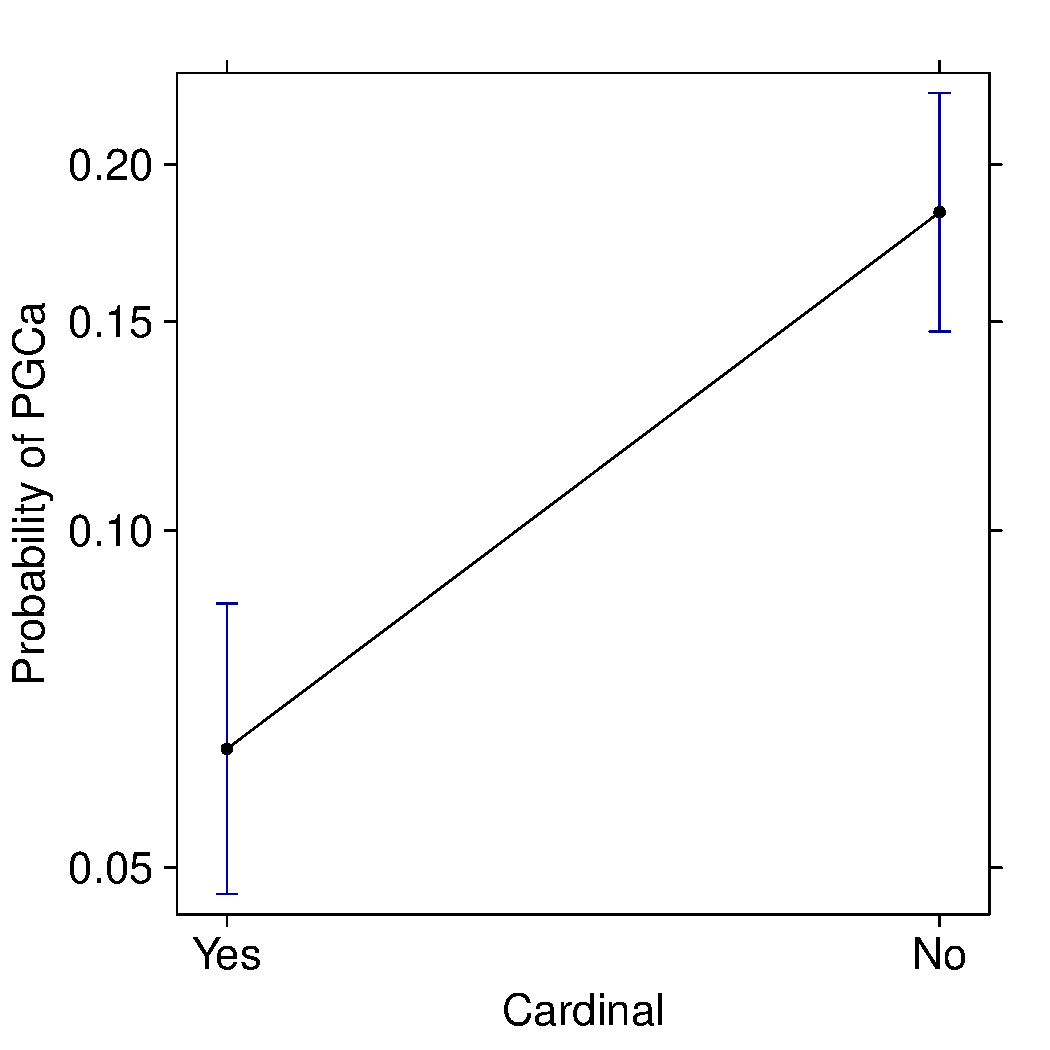
\includegraphics[width=0.5\textwidth]{../R/output/corpus_Cardinal}
  \caption{Effect plot for the regressor \textit{Cardinal}}
  \label{fig:eff:leftcontext}
\end{figure}

Figure~\ref{fig:eff:leftcontext} shows that cardinals indeed influence the choice of the alternant, and that cardinals have a strong tendency to co-occur with the \NACa.

The style-related proxy variables point in the expected direction.
Increased \textit{Badness} of the document favours the \NACa, and so does a lower density of genitives.
While these are merely proxies to style, this result can at least encourage future work into stylistic effects. 

The influence of \textit{Measurecase} is as predicted in previous analyses.
A measure noun in the dative favours the \PGCa\ (compared to the nominative, which is on the intercept).
Although \textit{Measurecase} is a nuisance variable in the context of this study, convergence with previous work strengthens its validity.

To close this section, I now compare the results of the pre-study and the main study.
Even though the non-alternating constructions are surely subject to additional constraints, the coefficients align neatly in many cases.
First of all, the intercepts encode a similar overall dominance of the NAC constructions (pre-study: -5.370; main study: -3.548).
For the \textit{Cardinal} effect, the coefficients 1.419 (pre-study) and 1.189 (main study) have the same sign and magnitude and mostly overlapping confidence intervals.
The levels of \textit{Measureclass} have comparable coefficients, although the divergence is larger.
In both studies, the non-referential measure nouns in the \textit{Physical} class (on the intercept) are most clearly associated with the NAC constructions.
Also, in both cases, the \textit{Container} class is closest to \textit{Physical} with the same sign and magnitude (pre-study: 0.445; main study: 0.252).
The main difference -- if we ignore the \textit{Rest} class which can be expected to show no clear tendency -- is that \textit{Amount} and \textit{Portion} are slightly closer together in their tendency to favour the PGC constructions in the pre-study (\textit{Amount} 1.597 and \textit{Portion} 1.782 in the pre-study vs.\ \textit{Amount} 0.831 and \textit{Portion} 1.217 in the main study).
The difference is not huge, and the overall order of the coefficients is the same.
The \textit{Genitives} effect also converges with -0.710 in the pre-study and -0.693 in the main study.
The two studies do not converge with respect to the \textit{Badness} variable, which is not significant in the pre-study.
However, it would be surprising if we achieved perfectly converging results given that even real effects are missed at certain rates in empirical studies.
In the case of \textit{Badness}, we see that even in the main study, the post-hoc effect size is small (-0.152), and thus even at the impressive sample size of roughly 5,000 in both studies, the effect might simply be too weak to be detected reliably.
Finally, the frequency effect \textit{Measurefreq} is detected in the main study but not in the pre-study, while the \textit{Kindfreq} effect is essentially absent in both studies.
In connection with this, it is revealing to look at the coefficients of determination.
In the pre-study, a much greater proportion of the variance is explained by taking the lemma random effects into account ($R^2_m=0.278$ and $R^2_c=0.566$) than it is in the main study ($R^2_m=0.409$ and $R^2_c=0.495$).
Thus, the frequency effect for measure lemmas might be swamped by the lemma random intercepts.
All things considered, the studies have shown that the predicted prototype and exemplar effects are reflected in usage data for both the alternating and the non-alternating constructions.
